\section{Demi-droite graduée (2 points)}

{\Large \textbf{Cet exercice est le seul à faire sur cette feuille}.} 

Voici une demi-droite graduée sur laquelle sont placés les points E et F.

\begin{center}
	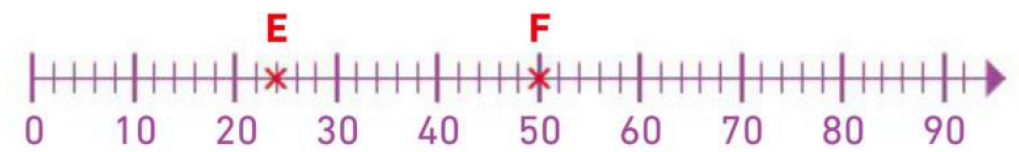
\includegraphics[scale=0.55]{img/droites2}
\end{center}

\begin{questions}
	\question[1] Quelles sont les abscisses des points $E$ et $F$ ?
	
	\question[1] Placer les points G et H, d'abscisses respectives 36 et 62.
\end{questions}